\section{Problem formulation}
\label{sec:formulation}

For a task \(t\) and an eligible primitive \(p\), the measured profile is
\begin{equation}
\label{eq:profile}
Y_{t,p} = (Q,\ C_{\mathrm{train}},\ C_{\mathrm{infer}},\ C_{\mathrm{api}},\ L_{p50},\ L_{p95},\ V).
\end{equation}
\(Q\) is macro-F1 on the frozen evaluation rows. Accuracy is stored and is not the quality coordinate. \(C_{\mathrm{train}}\) and \(C_{\mathrm{infer}}\) are local training time and inference time, in seconds. \(C_{\mathrm{api}}\) is API cost. \(L_{p50}\) and \(L_{p95}\) are per-example latency in milliseconds, excluding model load. \(V\) is the fraction of evaluation rows whose output is not exactly one legal label.

An invalid row is already incorrect for macro-F1. \(V\) is kept as its own coordinate because a legal wrong label and an output that is not a label are different failures, and macro-F1 does not say which occurred.

The prediction task is to estimate
\begin{equation}
\label{eq:predictor}
(\text{fingerprint of } t,\ \text{identity of } p) \mapsto \hat Y_{t,p}.
\end{equation}
\begin{figure}[htbp]
\centering
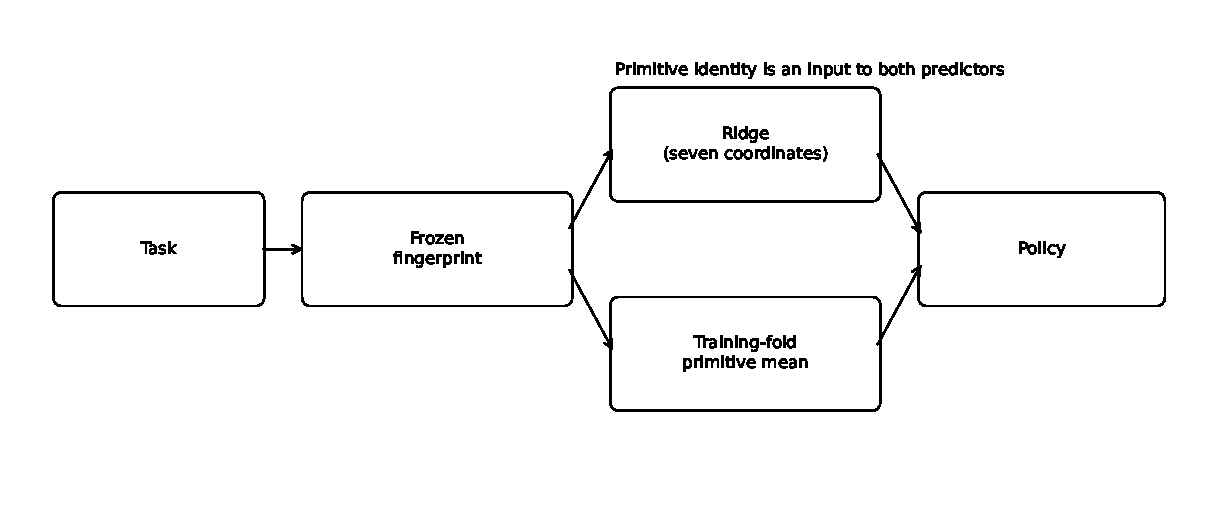
\includegraphics[width=0.95\linewidth]{figures/figure1_pipeline.pdf}
\caption{A task yields the frozen fingerprint. Primitive identity enters the ridge-based prediction coordinates and the training-fold primitive mean. A policy reads a predicted profile. There is no arrow from the task directly to a selected primitive.}
\label{fig:pipeline}
\end{figure}

The fingerprint is shared across primitives. The primitive identity is an intercept shift, with the classifier as the reference level. There is no product between a fingerprint coordinate and a primitive indicator. A policy may read \(\hat Y\) after it is predicted. The policy is not the training label. This split is deliberate: a single utility would encode a particular preference directly into the prediction target, and encoder-versus-LLM work already varies such weights~\citep{gonzalez2026}.

Higher \(Q\) is better. Lower cost, latency, and \(V\) are better. Ineligible pairs have no target. The rule is eligible only on SMS Spam. Measured zeros are retained as zeros. Training time for the rule, Laya, and Qwen is zero because those primitives are not trained on individual tasks. API cost is zero because no API was called.

\section{Computational primitives}
\label{sec:primitives}

All eligible primitives on a task see the same input string and the same label set.

\paragraph{Rule.}
A single regular expression was written and hashed before any scores were measured. It maps an SMS message to spam on a match and to ham otherwise. SHA-256 of the file bytes, including the trailing newline, is
\begin{center}
\texttt{264e288b89a430005de7b72fdfeb77862e46b23b7415c76df285e4e5e1a7f992}.
\end{center} The expression is not fit on labels. No other task receives a rule. A rule is not added to a 77-, 100-, or 151-way label set in response to a lower-scoring primitive.

\paragraph{Classifier.}
Word unigrams and bigrams, \path{min_df=2}, at most 30{,}000 features, sublinear term frequency, and logistic regression with the saga solver, \(C=1\), and at most 200 iterations. The iteration limit was not increased after a convergence warning on SMS Spam. Tasks with at most 100{,}000 fingerprint training rows use every such row (Cfull). Civil Comments, VitaminC, and ESCI are fit on a stratified 100{,}000-row subset (C100k). That cap is a frozen compute limit specified before evaluation. It is not a scarcity experiment and it is not the full-data classifier.

\paragraph{Typed decision model.}
\path{convaiinnovations/laya}, English router, one choice question. Criteria keys are the sorted training labels. Descriptions equal those keys. The instruction is ``Which label applies?'' Context limits are \path{max_len=2048} and \path{head_max_len=1024}. Inference was run on CPU. Load time is stored outside latency.

\paragraph{Generative model.}
\path{Qwen/Qwen2.5-0.5B-Instruct}, \path{do_sample} false, at most 32 new tokens, float16 on a GTX 1650 Ti. The prompt instructs the model to return exactly one label from a sorted list and not to provide an explanation. An output is valid only if, after stripping whitespace and at most one matching pair of surrounding quotes, it equals a legal label. All other outputs are classified as invalid. This configuration was not retuned after the invalid-output rates were observed.

\section{Task fingerprint}
\label{sec:fingerprint}

The fingerprint uses the task contract and the training split only. It does not use test labels, test examples, any primitive's outputs, or any coordinate of \(Y\). It does not use the benchmark name, the dataset identifier, or a subjective difficulty rating.

Token length is \mbox{\texttt{bert-base-uncased}} WordPiece without special tokens. The revision is
\begin{center}
\texttt{86b5e0934494bd15c9632b12f734a8a67f723594}.
\end{center}
Label-name similarity is mean-pooled \mbox{\texttt{all-MiniLM-L6-v2}}. The revision is
\begin{center}
\texttt{1110a243fdf4706b3f48f1d95db1a4f5529b4d41},
\end{center}
after lowercasing and replacing underscores and hyphens with spaces. Normalized entropy is Shannon entropy in nats divided by \(\ln K\).

The fingerprint features supplied to the predictor are, in order: \(\log_{10}\) of the training-row count, \(\log_{10}\) of \(K\), normalized entropy, \(\log_{10}\) of the max/min class-count ratio, \(\log_{10}\) of the minimum and median rows per class, \(\log_{10}\) of the median and P95 input lengths, and the mean and minimum label-name cosines. The relation code is supplied as a binary feature that is 1 for paired-text tasks. Primitive identity is supplied separately through primitive-indicator variables, with the classifier as the reference level. Input structure and evidence required make the same split of these eight tasks as that paired-text indicator, so they are not entered twice. The external-knowledge flag is false for every task. Documented shift is \path{unspecified} on four selector-training tasks and blank on VitaminC, so it is recorded and not used as a feature. The rule-eligibility flag is true only for SMS Spam and is not used as a fingerprint feature; primitive eligibility is determined by the primitive mask.

For Civil Comments and ESCI, the median and P95 input lengths are computed on a 20{,}000-row training sample drawn with seed \path{20260926}. Their imbalance uses the full training split. \Cref{tab:fingerprint-a,tab:fingerprint-b} report the fingerprint values used by the study.

\section{Experimental protocol}
\label{sec:protocol}

Evaluation rows are drawn before any fit. If the official test split contains at most 1{,}000 rows, all rows are used; otherwise, 1{,}000 rows are sampled without replacement. PubMedQA's test half has 500 rows, so its evaluation count is 500. Every other task in \cref{tab:performance} has 1{,}000 evaluation rows.

The ridge specification was frozen before this fit. Each learned coordinate uses \path{Ridge(alpha=1)} with an intercept. API cost is fixed at zero, and training-time prediction is fit only on classifier rows because the other primitives are not trained on individual tasks. Numeric fingerprint columns are standardized with the population mean and standard deviation of the training tasks in that fold. A column with zero variance is set to 0, including on the held-out task. Primitive indicators are not standardized. Predictions of \(Q\) and \(V\) are clipped to \([0,1]\). Time coordinates are clipped at 0. The penalty parameter was not tuned. No interaction was added after the errors were seen. Training time for the rule, Laya, and Qwen is fixed at zero because these primitives are not trained on individual tasks.

The baseline ignores the fingerprint. For each primitive present in the training tasks, it predicts the arithmetic mean of that primitive's measured coordinate. An unseen primitive is not predicted and is not imputed from another primitive. On the security holdout, SMS Spam is removed, so the rule has no training-fold mean and is therefore not predicted.

Task-level error is the mean absolute error across eligible primitives that both predictors can fill. Coordinates are not averaged into one score. A negative difference means the ridge prediction was closer.

Policies run after a vector exists. Always-Qwen, always-classifier, always-Laya, and the mask default do not read a vector. The mask default selects the rule when it is eligible and the classifier otherwise. The remaining policies read either a predicted vector or, for the oracle analysis, the measured vector. The measured vector is not a deployable predictor. The policies are: highest macro-F1; lowest \(L_{p50}\); equal weights \(U=\tilde Q-\tilde C_{\mathrm{infer}}-\tilde L_{p50}\); shared weights \(U=\tilde Q-\tfrac12\tilde C_{\mathrm{infer}}-\tfrac12\tilde L_{p50}\). Tildes are min-max maps whose minimum and maximum come from the training tasks of that fit, not from the held-out task. Ties break in the order rule, classifier, decision model, generative model. \(V\) is reported with the chosen primitive and is not given a weight.

Family labels are taken directly from the screening record and are not used as features. Intent holds out Banking77 and CLINC150 plus together. Verification holds out PubMedQA and VitaminC together. Moderation, security, and business/legal each hold out one task. For the e-commerce holdout, the predictor is fit on all seven selector-training tasks and evaluated on ESCI. ESCI does not enter any fit, any primitive mean, any standardization, or any utility range. A random 70/15/15 split of tasks is not run. Seven selector-training tasks are insufficient to support a meaningful 70/15/15 task-level split.

Example-level uncertainty concerns variation in a score across the evaluation rows of a single dataset. Task-level uncertainty concerns variation across tasks. Family-level uncertainty would require multiple tasks in each held-out family and several tasks left behind that still represent the fingerprint's informative features. This design has eight tasks. Three family holdouts are single-task holdouts. The verification holdout removes both paired-text training tasks, so that feature has no variance and is zeroed. We do not report \(p\)-values. A count such as ``5 of 8'' is a description of this sample, not a population rate.
